\section{Reproduction notes}\label{app:repro}
All code, result files and run commands are in the accompanying repository: \texttt{src/} (library), \texttt{scripts/} (experiment runners), \texttt{results/} (CSV files and a column guide), \texttt{figtab/} (one script per figure and table, with input files recorded in \texttt{figtab/MANIFEST.md}) and \texttt{REPRODUCE.md} (environment and package versions, data sources and versions, seeds, commands, expected run times, and the map from each exhibit to its script). Data: CIFAR-10 (copy from the Hugging Face dataset \texttt{uoft-cs/cifar10}, a fixed revision recorded in \texttt{REPRODUCE.md}; no licence stated by the source) and CIFAR-10H human label distributions (no licence stated); both are cited in \texttt{REPRODUCE.md}. No forbidden material was encountered; this is recorded there.


\paragraph{Exhibit map.} Numbering in the paper differs from the file names in \texttt{figures/} and \texttt{tables/}: Fig.~\ref{fig:beta} \texttt{fig1\_beta\_law}; Fig.~\ref{fig:size} \texttt{fig2\_size}; Fig.~\ref{fig:cond} \texttt{fig3\_conditional}; Fig.~\ref{fig:null} \texttt{fig5\_null\_spread}; Fig.~\ref{fig:ncal} \texttt{fig4\_ncal}; Fig.~\ref{fig:delta} \texttt{fig6\_delta\_method}; Fig.~\ref{fig:shift} \texttt{fig7\_shift}; Fig.~\ref{fig:sizevol} \texttt{fig2\_size\_volume}; Fig.~\ref{fig:eps} \texttt{fig8\_eps\_sensitivity}; Table~\ref{tab:e1} \texttt{tab2\_e1\_headline}; Table~\ref{tab:e2} \texttt{tab3\_e2\_labelsets}; Table~\ref{tab:e3} \texttt{tab4\_e3\_cifar10h}; Tables~\ref{tab:gridd}--\ref{tab:gridro} \texttt{tabA\_e1\_grid\_*}. Each is produced by the script of the same stem in \texttt{figtab/} from the result files named in \texttt{figtab/MANIFEST.md}.
\section{Additional E1 exhibits}\label{app:e1}
\begin{figure}[h]
\centering
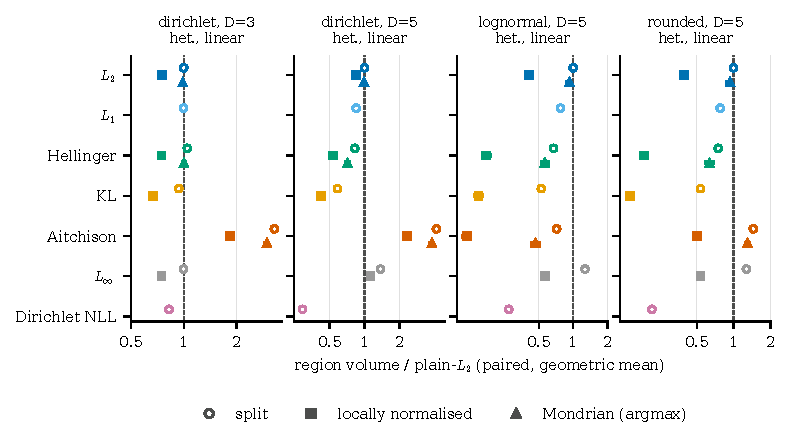
\includegraphics[width=\linewidth]{fig2_size_volume.pdf}
\caption{As Fig.~\ref{fig:size} with the Lebesgue volume of the region (Monte-Carlo) instead of the mass, in four configurations with $K\le5$ (Dirichlet $K=3,5$; logistic-normal and rounded $K=5$), where volume is computable.}\label{fig:sizevol}
\end{figure}
\begin{figure}[h]
\centering
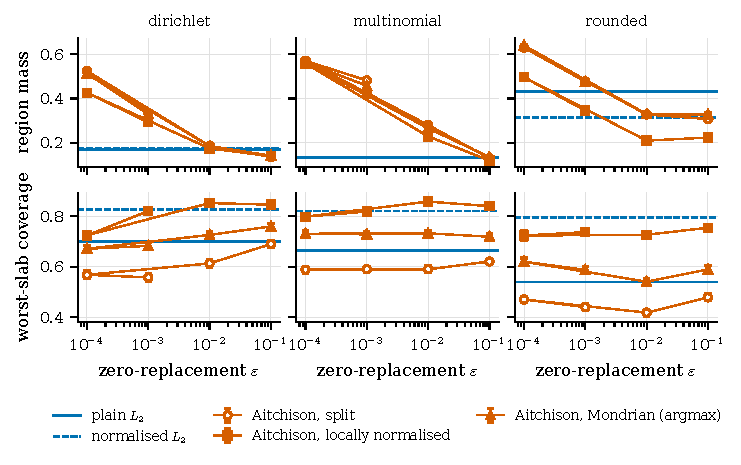
\includegraphics[width=\linewidth]{fig8_eps_sensitivity.pdf}
\caption{Sensitivity of the plain Aitchison score to the zero replacement $\varepsilon$ ($K=5$, heteroscedastic, linear predictor, $n_{\mathrm{cal}}=500$, $100$ replicates, $95\%$ $t$-intervals). Top: region mass; bottom: worst-slab coverage. Blue lines: plain and normalised $L_2$, independent of $\varepsilon$.}\label{fig:eps}
\end{figure}
\begin{table}[h]
\centering\scriptsize
\caption{All $12$ Dirichlet-noise configurations of the E1 grid ($n_{\mathrm{cal}}=500$, $100$ replicates; means; largest $95\%$ half-widths: oracle gap $0.004$, wsc $0.015$, mass $0.01$). cov.\ range: minimum--maximum over the $16$ methods of mean coverage. Oracle gap and wsc for plain and normalised $L_2$; mass for plain $L_2$, KL, Aitchison and Dirichlet NLL. Logistic-normal, multinomial and rounded: Tables~\ref{tab:gridln}--\ref{tab:gridro}.}\label{tab:gridd}
\input{../tables/tabA_e1_grid_dirichlet}
\end{table}
\begin{table}[h]
\centering\scriptsize
\caption{As Table~\ref{tab:gridd}, logistic-normal noise.}\label{tab:gridln}
\input{../tables/tabA_e1_grid_lognormal}
\end{table}
\begin{table}[h]
\centering\scriptsize
\caption{As Table~\ref{tab:gridd}, multinomial noise.}\label{tab:gridmn}
\input{../tables/tabA_e1_grid_multinomial}
\end{table}
\begin{table}[h]
\centering\scriptsize
\caption{As Table~\ref{tab:gridd}, rounded logistic-normal noise.}\label{tab:gridro}
\input{../tables/tabA_e1_grid_rounded}
\end{table}

\section{Further exhibits for Section~\ref{sec:exp}}\label{app:more}
\begin{figure}[h]
\centering
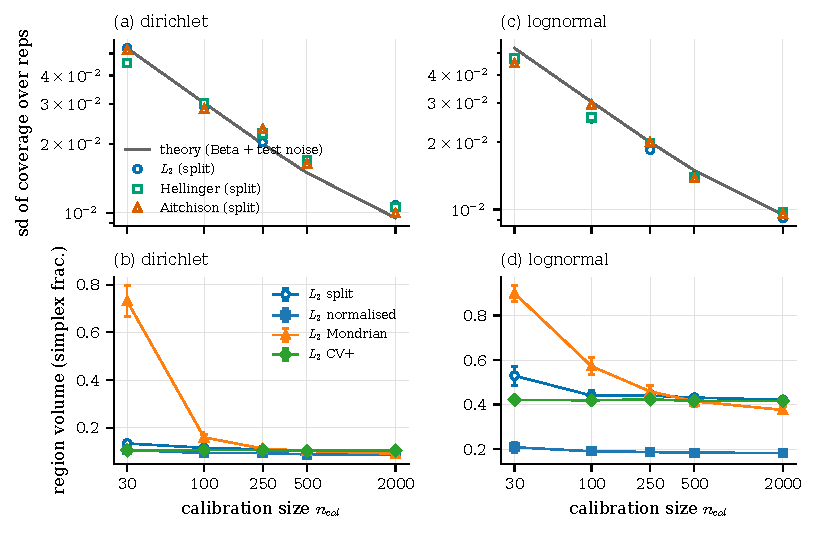
\includegraphics[width=\linewidth]{fig4_ncal.pdf}
\caption{Calibration size ($K=5$, heteroscedastic, linear predictor, $100$ replicates per point). (a,c) Standard deviation over replicates of test coverage; line: $\sqrt{\mathrm{Var}\,\mathrm{Beta}+0.09/2000}$. (b,d) Median region volume (fraction of the simplex) with $95\%$ $t$-intervals for split, locally normalised and Mondrian $L_2$ and for CV+; $n_{\mathrm{cal}}=500$ points come from the main grid.}\label{fig:ncal}
\end{figure}
\begin{figure}[h]
\centering
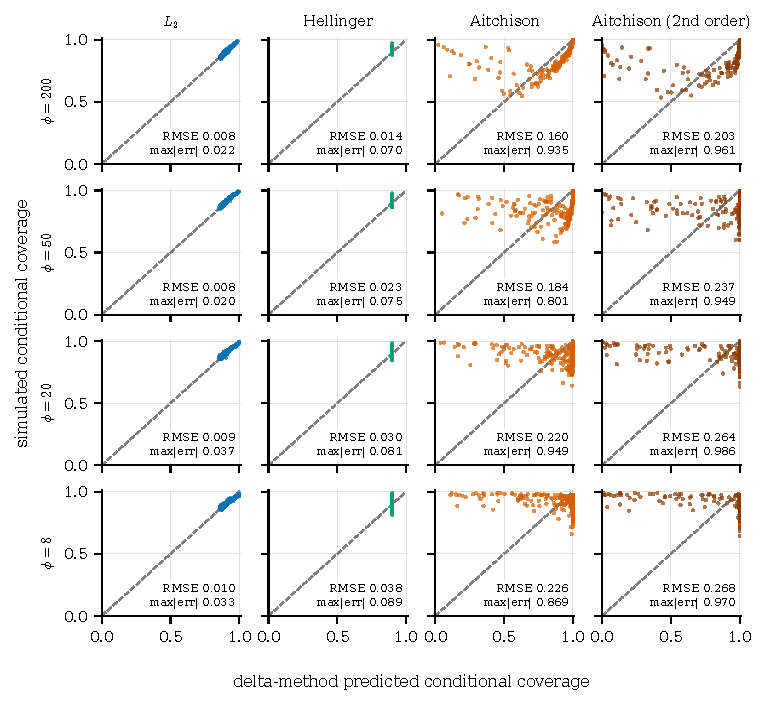
\includegraphics[width=\linewidth]{fig6_delta_method.pdf}
\caption{Delta-method prediction (horizontal) against simulated pointwise conditional coverage (vertical) of the marginal threshold at nominal $0.9$, $K=5$, Dirichlet noise, oracle mean predictor. Rows: precision $\phi$; columns: score (Aitchison in first-order and second-order moment versions). Dashed: identity.}\label{fig:delta}
\end{figure}
\begin{table}[h]
\centering\small
\caption{CIFAR-10H as a composition-valued response, $12$-epoch CNN softmax, $\alpha=0.1$, $n_{\mathrm{cal}}=1000$, $100$ random splits; mean $\pm$ half-width of the $95\%$ $t$-interval. mass: share of $300$ other images' human distributions inside the region; ambig.\ min / conf.\ min: coverage in the worst of $5$ equal-mass bins of the entropy of the human distribution / of the CNN's top-1 probability; wsc: worst-slab coverage ($\delta=0.1$).}\label{tab:e3}
\resizebox{\linewidth}{!}{\input{../tables/tab4_e3_cifar10h}}
\end{table}
\begin{figure}[h]
\centering
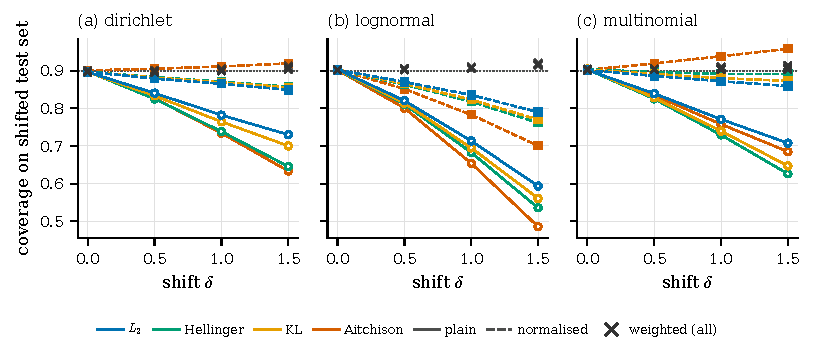
\includegraphics[width=\linewidth]{fig7_shift.pdf}
\caption{Test coverage under covariate shift of size $\delta$ towards noisier inputs ($K=5$, heteroscedastic, linear predictor, $n_{\mathrm{cal}}=500$, $100$ replicates). Lines: ordinary split conformal (solid: plain, dashed: locally normalised) with $95\%$ $t$-intervals; crosses: weighted split conformal with the exact likelihood ratio.}\label{fig:shift}
\end{figure}
\begin{table}[h]
\centering\small
\caption{E1, $K=5$, heteroscedastic, linear predictor, $n_{\mathrm{cal}}=500$, means over $100$ replicates (largest $95\%$ half-widths: coverage $0.004$, wsc $0.016$, oracle gap $0.004$, mass $0.009$). wsc: worst-slab coverage; or.\ gap: oracle conditional-coverage gap (null floor $0.011$--$0.025$); mass: region mass. Bold: best of the $15$ methods in the column (no significance claim).}\label{tab:e1}
\input{../tables/tab2_e1_headline}
\end{table}
